\begin{wrapfigure}{r}{4.4cm}
	\begin{tikzpicture}
	\def\IA{(0,0) circle (2.2cm)}
	\def\AM{(270:1.0cm) circle (1.2cm)}
	\def\AP{(270:1.52cm) circle (.675cm)}
	\draw \IA node[above]{\small $\overset{\text{Inteligencia artificial}}{}$};
	\draw \AM node[above]{\scriptsize $\overunderset{\text{Aprendizaje}}{\text{maquinal}}{}$};
	\draw \AP node{\tiny $\overunderset{\text{Aprendizaje}}{\text{profundo}}{}$};
	\end{tikzpicture}\caption[Inteligencia Artificial]{AP$\subset$AM$\subset$IA}
\end{wrapfigure}\label{fig:AI}\subsection {AI, ML, NLP}\label{subsec:intela}
\emph{Inteligencia artificial (IA)} es ``el esfuerzo por automatizar tareas intelectuales normalmente realizadas por humanos''\cite{cho18}, de este campo general se desprenden el \emph{aprendizaje maquinal (AM)} y \emph{aprendizaje profundo (AP)}.
%\begin{figure}[H]\centering
%\begin{tikzpicture}
%\def\IA{(0,0) circle (1.5cm)}
%\def\AM{(270:.7cm) circle (.75cm)}
%\def\AP{(270:1.025cm) circle (.375cm)}
%\draw \IA node[above]{IA};
%\draw \AM node[above]{AM};
%\draw \AP node{AP};
%\end{tikzpicture}
%\caption{Aprendizaje profundo (AP), es un subcampo del aprendizaje maquinal (AM), que a su vez es un subcampo de la inteligencia artificial (IA)\cite{cho18}.}\label{fig:AI}
%\end{figure}

Tom Mitchell \cite{mich19} define aprendizaje maquinal como ``un programa de computadora aprende de experiencia $E$ con respecto a una tarea $T$ y una medición de rendimiento $P$, si su rendimiento en $T$, medido por $P$, mejora con $E$.''

A diferencia del paradigma clásico de programación donde los humanos introducen datos y órdenes para procesarlos, un sistema de aprendizaje maquinal no se programada explícitamente, se introducen muchos ejemplos relevantes a una tarea (datos y respuestas esperadas) con los que es entrenado y si encuentra una estructura estadística en ellos, genera una regla para automatizar la tarea.

El \emph{procesamiento de lenguaje natural}, es el conjunto de métodos para hacer accesible el lenguaje humano a las computadoras\cite{eise19}. Toma conocimientos de muchas tradiciones intelectuales, como lingüística Existen dos enfoques en lo que debe ser su tarea central: 
\begin{itemize}
	\item Entrenar sistemas de principio a fin para que transmuten texto sin procesar en cualquier estructura deseada.
	\item Transformar texto en una pila de estructuras lingüísticas de uso general que en teoría deben poder soportar cualquier aplicación.
\end{itemize}
Dos de los módulos básicos de NLP son \emph{búsqueda} y \emph{aprendizaje} con los que se puede resolver muchos problemas que podemos describir en la siguiente forma matemática
\begin{equation}
\begin{matrix}
\hat{y}=argmax\Psi(x,y;0),\\
y\in Y(x)
\end{matrix}
\end{equation}
donde,
\begin{itemize}
	\item $x$ es la entrada, un elemento de un conjunto $X$.
	\item $y$ es el resultado, un elemento de un conjunto $Y$.
	\item $\Psi$ es una función de puntuación (también conocida como \emph{modelo}), que va desde el conjunto $X\times Y$ hasta los números reales.
	\item $\emptyset$ es el vector de parámetros para $\Psi$.
	\item $\hat{y}$ es el resultado previsto, que es elegido para maximizar la función de puntuación.
\end{itemize}
El módulo de búsqueda se encarga de computar el $argmax$ de la función $\Psi$, es decir, encuentra el resultado $\hat{y}$ con la mejor puntuación con respecto a la entrada $x$. El módulo de aprendizaje encuentra los parámetros $\theta$ por medio del procesamiento de grandes conjuntos de datos de ejemplos etiquetados ${\{(x^i,y^i)\}}_{i=1}^{N}$.